% !TEX root = ./main.tex

%\secmoveup
\section{Experimental results}
\label{sec:experiment}
%\textmoveup


We present empirical evaluations for the trajectory recommendation task % in Section~\ref{sec:trajrec}.
%Results are reported 
on real-world datasets of photo tours,
created from the publicly available YFCC100M corpus~\cite{thomee2016yfcc100m} as described below.
%LX - this is verbose
%We now present evaluations assessing the viability of our structured prediction approach
%for the trajectory recommendation task discussed in Section~\ref{sec:trajrec}.
%LX - don't be a spoiler!
%On a real-world dataset of photo tours, our methods are shown to significantly outperform
%a number of non-structured baselines or those that do not take into account the recommendation setting.


%\secmoveup
\subsection{Photo trajectory datasets}
\label{sec:dataset}
%\textmoveup

% experiment protocol: Nested cross-validation with Monte-Carlo cross-validation for the inner loop
%We assess the recommendation performance %methods developed in Section~\ref{sec:trajrec}
We used the trajectory data %\footnote{\url{https://bitbucket.org/d-chen/tour-cikm16}} % double-blind! 
extracted from Flickr photos for the cities of Osaka, Glasgow and Toronto~\cite{ijcai15,cikm16paper}.
Each dataset comprises of a list of trajectories, being a sequence of points-of-interest (POI),
as visited by various Flickr users and recorded by the geotags in photos.
%Photos that are nearby in time and space are grouped, \rev{mapped to POIs,} and then segmented by eight hours of time gap. Visits \rev{with} %that only include
%a single POI are excluded.
%We use 12 behavioural and geographical features to describe each POI and pairs of POIs (see supplement).
Table~\ref{tab:data} summarises the profile of each dataset.
We see that most queries have more than one ground truth, making the sequence recommendation setting relevant. Further, each query has an average of 4-9, and a maximum of 30-60 trajectories (details in Figure~\ref{fig:hist_query}).
The histograms of trajectory length are shown in Figure~\ref{fig:hist_length}.
% All datasets are sparse in user activity,
% i.e.,
In all datasets,
each user has on average less than two trajectories.
This makes user-specific recommendation impractical, and also undesirable because
%of the domain being urban locations
a user would want different recommendations given different starting locations, and not a static recommendation no matter where she is.
The sparsity of this dataset presents a barrier for large-scale evaluations.
%Music playlist datasets are larger, but recent results show that sequencing information does not affect the data likelihood~\cite{chen2012playlist}.

% dataset stats
%\begin{table}[t]
\begin{table*}[t]
    \centering
	%\begin{minipage}[t]{\linewidth}
	%	\resizebox{\linewidth}{!}{
	%	\setlength{\tabcolsep}{4pt} % tweak the space between columns
		\small
		\begin{tabular}{lllll|ccc|cc} \hline %{l*{9}{c}} \hline
		\textbf{Dataset} & \textbf{\#Traj} & \textbf{\#POIs} & \textbf{\#Users} & \textbf{\#Queries} & \textbf{\#GT=1} & \textbf{\#GT$\in [2,5]$} & \textbf{\#GT$>$5} & \textbf{\#shortTraj} & \textbf{\#longTraj} \\ \hline
		Osaka            & 186              & 26              & 130              & 47                 & 17              & 22                      & 8                 & 178                     & 8  \\
		Glasgow          & 351              & 25              & 219              & 64                 & 23              & 22                      & 19                & 336                     & 15 \\
        Toronto          & 977              & 27              & 454              & 99                 & 30              & 33                      & 36                & 918                     & 59 \\
		\hline
		\end{tabular}%
		%}
		\captionof{table}{Statistics of trajectory datasets.
        Including the number of trajectories (\#Traj), POIs (\#POIs), users (\#Users), queries (\#Queries);
        the number of queries with a single (\#GT=1), 2-5 (\#GT$\in$[2,5]), or more than 5 (\#GT$>$5) ground truths;
        and profile of trajectory length, \ie less than 5 (\#shortTraj) and more than 5 POIs (\#longTraj).
        }
		\label{tab:data}
	%\end{minipage}
    %\captionmoveup
	%%\quad
	%%\begin{minipage}[t]{0.45\linewidth}
	%%	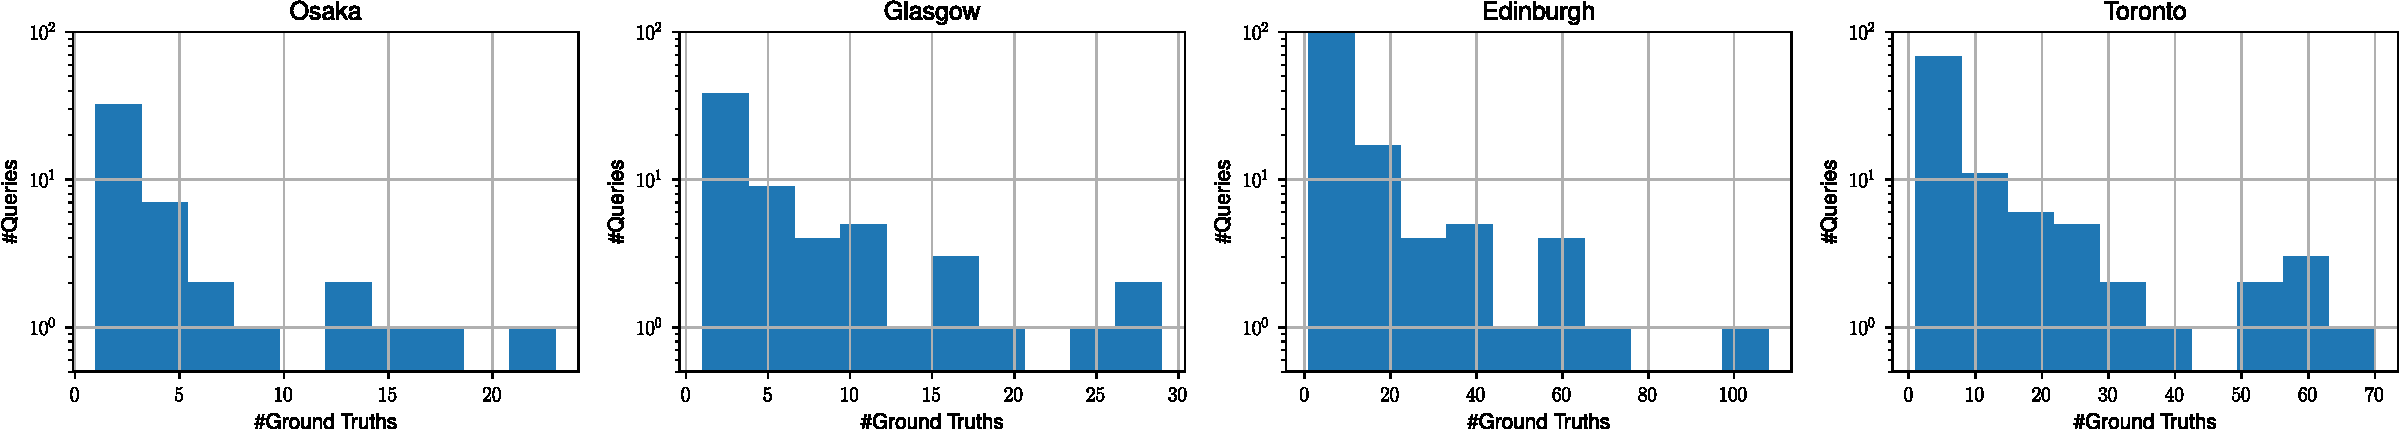
\includegraphics[scale=0.25]{hist_query.pdf}
	%%    \captionof{figure}{\# of trajectories per query.}
	%%    \label{fig:image}
    %%\end{minipage}
\end{table*}

% histogram of #ground truth
\begin{figure}[t]
	\centering
	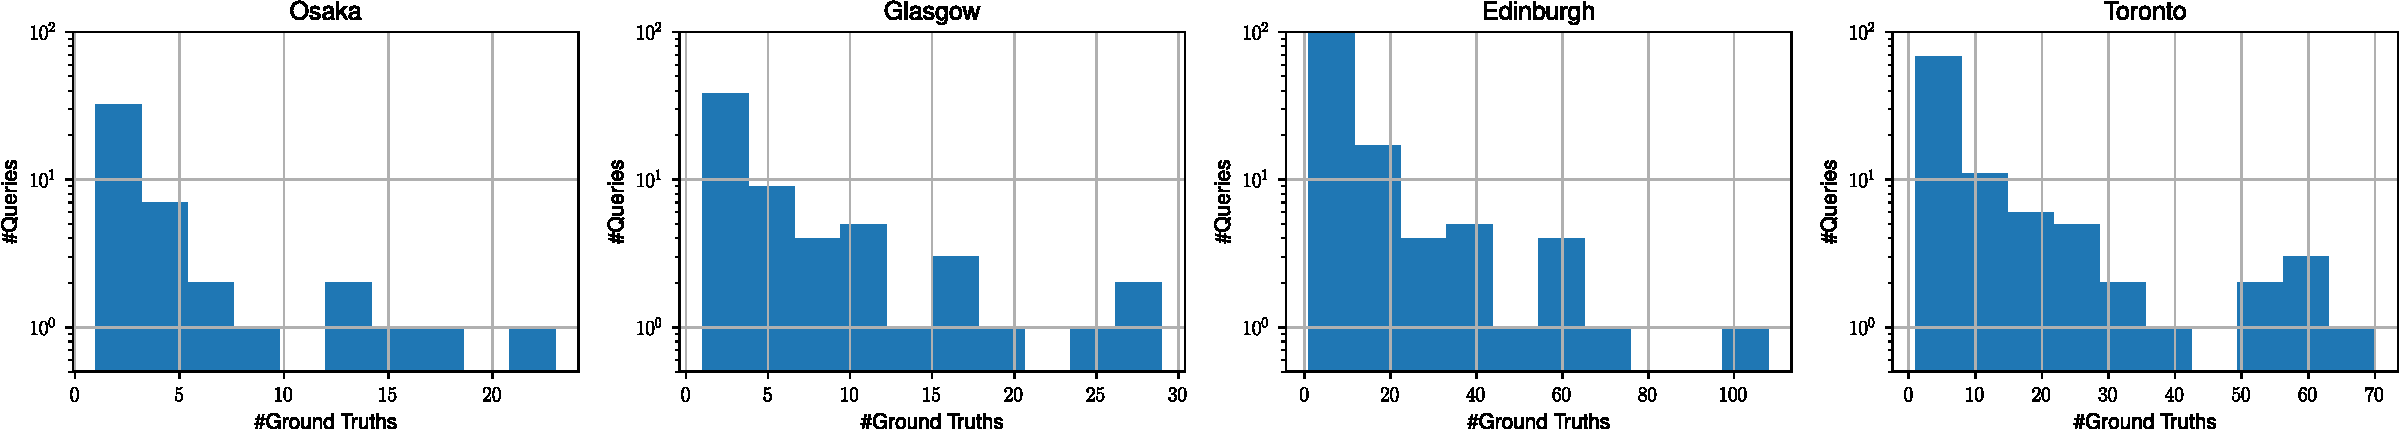
\includegraphics[width=\linewidth]{hist_query.pdf}
	\caption{Histograms of the number of trajectories per query.}
	\label{fig:hist_query}
\end{figure}

% histogram of trajectory length
\begin{figure}[t]
	\centering
	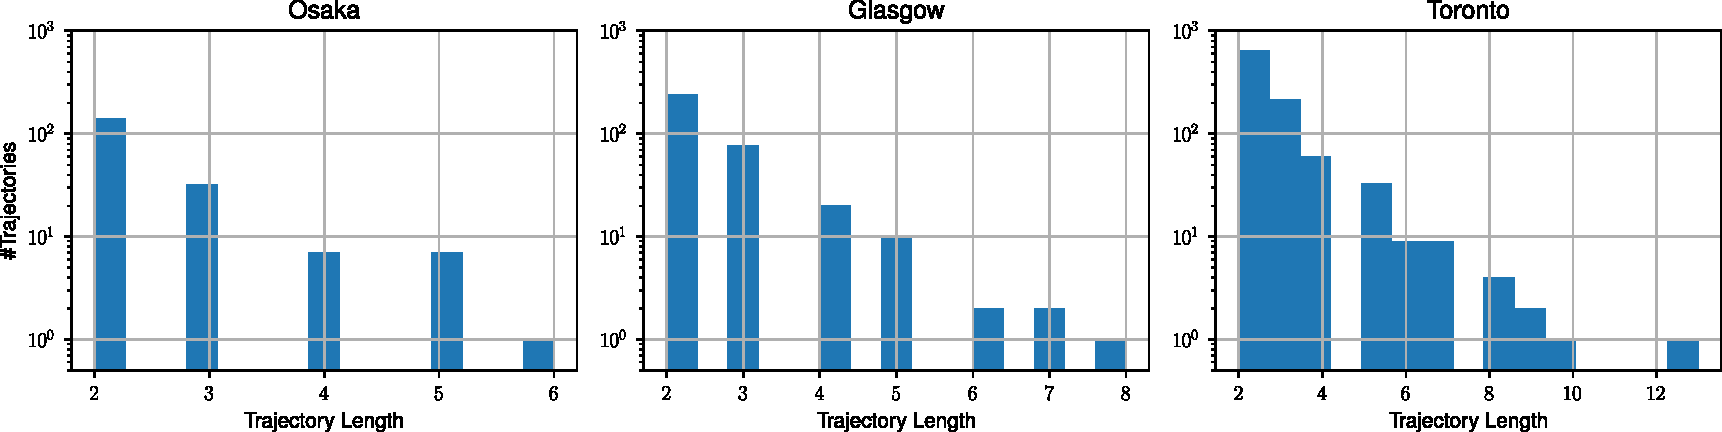
\includegraphics[width=\linewidth]{hist_length.pdf}
	\caption{Histograms of trajectory length.}
	\label{fig:hist_length}
\end{figure}




%LX - this doesn't belong here. first summarize what's in the dataset, then
%From Table~\ref{tab:data}, %%and Figure~\ref{fig:hist},
%we see that each distinct query %, %comprising of start POI and a desired trip length,
%has an average of 4-9, and a maximum of 30-60 trajectories.
%LX - delete? the sentence below is redundant and has no new info??
%Therefore, evaluation is carried out on the problem of recommending trajectories given a query.

%\newsavebox\tmpbox

% % dataset stats
% \begin{table}[t]
% 	\sbox\tmpbox{%
% 		\resizebox{0.4\linewidth}{!}{
% 		\setlength{\tabcolsep}{4pt} % tweak the space between columns
% 		\small
% 		\begin{tabular}{l*{5}{c}} \hline
% 		\textbf{Dataset} & \textbf{\#Traj.} & \textbf{\#POIs} & \textbf{\#Users} & \textbf{\#Queries} & \textbf{AvgLenth} \\ \hline
% 		Osaka            & 186              & 26              & 130              & 47                 & 2.4 \\
% 		Glasgow          & 351              & 25              & 219              & 64                 & 2.5 \\
% 		\hline
% 		\end{tabular}%
% 		}
% 	}%
%   \renewcommand*{\arraystretch}{0}
%   \begin{tabular*}{\linewidth}{@{\extracolsep\fill}p{\wd\tmpbox}p{40mm}@{}}
%     \usebox\tmpbox &
%     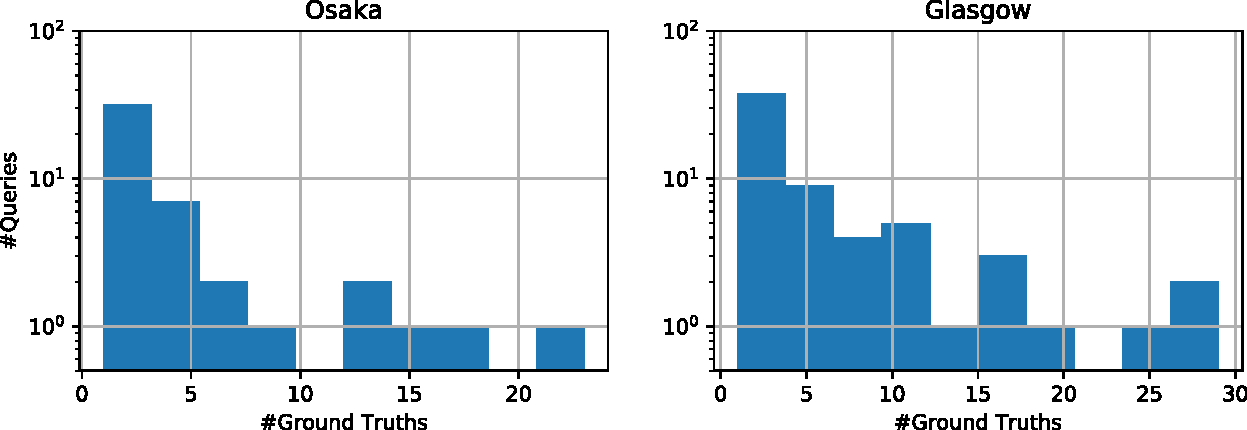
\includegraphics[scale=0.4]{hist.pdf} \\
%     \caption{Statistics of trajectory dataset.}
%     \label{tab:data}
%     &
%     \captionof{figure}{Histograms of the number of trajectories per query.}
%     \label{fig:image}
%   \end{tabular*}
% \end{table}


%\secmoveup
\subsection{Evaluation setting}
\label{ssec:methods}
%\textmoveup

We compare our methods to the following four baselines:
\begin{itemize}[leftmargin=0.125in]%%\itemmoveup
%\parskip -.05em
\item The \textsc{Random} baseline recommends a sequence of POIs by sampling uniformly at random from the whole set of POIs
      (without utilising any POI or query related features). 

\item The stronger \textsc{Popularity} baseline recommends the top-$l$ most popular POIs,
      \ie the POIs visited by the most number of users in the training set.

\item \textsc{PoiRank}~\cite{cikm16paper}
      %is a generalisation of \textsc{Popularity} which
      augments \textsc{Popularity} with a number of POI-query features (see supplement),
      and trains a RankSVM %~\eqref{eq:ranksvm} 
      to learn a score for each POI.
      A trajectory is constructed from the top-$l$ scored POIs.

\item \textsc{Markov}~\cite{cikm16paper} learns a Markov chain by factorising the transition probabilities between POIs 
      according to %a number of 
      pairwise features (see supplement). 

\end{itemize}%\itemmoveup

%LX - this is very long-winded
%To assess the viability of our structured prediction approach, and the necessity of our two extensions (normalising the loss per query and disallowing loops), we consider the following structured methods: %the following versions of our structured prediction methods:
We consider four variants of sequence recommendation, starting with a structured prediction model, then incorporating multiple ground truths, and finally path constraints:
\begin{itemize}[leftmargin=0.125in]
%\item The structured prediction ({\sc SP}) method employs the vanilla structured SVM framework in order to learn a score for trajectories given a query.
\item The SP and SR methods, %described in Section~\ref{ssec:sr}, 
      using both POI-query features and pairwise features (see supplement).
%\item The structured recommendation ({\sc SR}) method extends the {\sc SP} method by additionally incorporating multiple ground truths into
%      forming the constrai{}nts and adding them in cutting-plane algorithm,
%      described in Section~\ref{ssec:sr}.
	%performing normalisation of the loss function per query,
	%so that we do not attempt to distinguish between multiple ground truths for the same query.

\item {\sc SPpath} and {\sc SRpath}, %described in Section~\ref{ssec:training} 
      using the same features as SP and SR, but with path constraints for model learning.
\end{itemize}%\itemmoveup
We reiterate that irrespective of the training procedure, \textsc{SP}, \textsc{SR},
\textsc{SPpath} and \textsc{SRpath} all predict paths.
%use prediction procedures that eliminate loops. % subtours.

%LX - not clear what the sentence below is trying to say, delete.
%All above methods take into account the specified start location properly.

% LX - why not have one long subsection rather than two short ones?
%\secmoveup
%\subsection{Evaluation procedure}
%\textmoveup


%We then evaluate the performance of each algorithm using leave-one-query-out cross validation.
% LX - remove extra words!!
We evaluate each algorithm using leave-one-query-out cross validation.
That is, holding out all the relevant trajectories for each query $\x\pb{i}$ (\ie $\{\y\pb{ij}\}_{j=1}^{n_i}$) in each round.
%where in each iteration of this procedure,
%one query and its associated trajectories serves as a test point, with all other trajectories for training.
%(Note that without this query aggregation, there will be considerable overlap between the train and test set, and simple nearest neighbour methods will be hard to outperform.)
% model selection (Monte Carlo CV) (with query aggregation): 90/10 random split for 5 times
The regularisation constant $C$ is tuned using Monte Carlo cross validation %~\cite{burman1989comparative} 
on the training set.
We use three performance measures for POIs, sequences and ordered lists.
%We use three different measures to compare algorithm performances.
The {\bf F$_1$ score on points}~\cite{ijcai15} computes F$_1$ on the predicted versus seen points
without considering their relative order.
The {\bf F$_1$ score on pairs}~\cite{cikm16paper} %is proposed to
can mitigate this by computing F$_1$ on all ordered pairs in the predicted versus ground truth sequence. %%It is 1 iff both sequences agree completely.
The well-known rank correlation {\bf Kendall's $\tau$}~\cite{agresti2010analysis}
computes the ratio of concordant (correctly ranked) %pairs 
minus discordant pairs, over all possible pairs after accounting for ties.%taking care of ties.
%$\frac{1}{2}l(l-1)$) pairs  %DW: this is not correct

Sequence recommendation methods perform ranking on a very large label set (of size $m^l$).
We report results on the {\em best of top $k$}~\cite{russakovsky2015imagenet}:
for all methods, % described in Section~\ref{ssec:methods},
we predict the top $k$ trajectories\footnote{To get $k$ paths, the list Viterbi algorithm normally searches a long list which contains sequences with loops.}
and then report the best match of any in the top $k$ to any trajectory in the ground truth set.

To obtain top-$k$ recommendations with \textsc{Random}, we independently repeat $k$ times.
To perform top-$k$ prediction with \textsc{Popularity}, \textsc{PoiRank} and \textsc{Markov},
we exploit the 
%same approach 
list Viterbi algorithm
that was used to deal with multiple ground truths.
For \textsc{Popularity}, the score of a path is the accumulated popularity of all POIs in the path;
for \textsc{PoiRank} and \textsc{Markov}, the score of a path is the likelihood
(the ranking scores for POIs are first transformed into a probability distribution using the softmax function, as described in~\cite{cikm16paper}).

\eat{
As described previously, our methods are capable of recommending not merely a single trajectory,
but rather a list of trajectories.
While one can take the top recommended trajectory as the prediction,
this ignores the fact that there are likely multiple plausible trajectories for any given query.
Thus, for each performance measure $\mathrm{perf}$,
we take the maximum over all trajectories,
i.e.,
\begin{equation*}
%\tau_b^{(i)} =
\mathrm{perf}^{(i)}( \mathbf{y}, \hat{\mathbf{y}} ) =
\max_{(\mathbf{y}, \hat{\mathbf{y}}) \in \{\mathbf{y}^{(ij)}\}_{j=1}^{N_i} \times \{\hat{\mathbf{y}}^{(ij)}\}_{j=1}^k}
%\tau_b(r_\mathbf{y}, r_{\hat{\mathbf{y}}}),
\mathrm{perf}(\mathbf{y}, {\hat{\mathbf{y}}}),
\end{equation*}
where $\{\mathbf{y}^{(ij)}\}_{j=1}^{N_i}$ are the ground truths for query $\mathbf{x}^{(i)}$ and
$\{\hat{\mathbf{y}}^{(ij)}\}_{j=1}^k$ are the top-$k$ recommendations.
}

%\secmoveup
\subsection{Results and discussion}
\label{sec:result}
%\textmoveup

% !TEX root = ./main.tex

\begin{table*}[t]\captionmoveup
     \caption{Results on trajectory recommendation datasets on best of top-10.
     %The top three rows are baselines, and the bottom four are the methods proposed in this paper.
     Higher scores are better for all metrics. Bold entries: \textbf{best} performing method for each metric; italicised entries: the \textit{second best}.
     }
     \label{tab:result}
     \centering
%%     \setlength{\tabcolsep}{3pt} % tweak the space between columns
%%     \small
     \resizebox{\linewidth}{!}{
%%     \begin{tabular}{l|cc|cc|cc} \hline
%%                         & \multicolumn{2}{|c}{\textbf{Kendall's $\tau$}}
%%                         & \multicolumn{2}{|c}{\textbf{F$_1$ score on points}}
%%                         & \multicolumn{2}{|c}{\textbf{F$_1$ score on pairs}} \\ \cline{2-7}
%%                         & Osaka & Glasgow
%%                         & Osaka & Glasgow
%%                         & Osaka & Glasgow \\ \hline
%%     \textsc{Random}     & $0.685\pm0.035$ & $0.703\pm0.029$
%%                         & $0.703\pm0.032$ & $0.731\pm0.026$
%%                         & $0.451\pm0.057$ & $0.495\pm0.046$ \\
%%     \textsc{Popularity} & $0.768\pm0.038$ & $0.748\pm0.036$
%%                         & $0.786\pm0.034$ & $0.771\pm0.033$
%%                         & $0.626\pm0.055$ & $0.623\pm0.051$ \\
%%     \textsc{PoiRank}    & $0.787\pm0.037$ & $0.830\pm0.029$
%%                         & $0.804\pm0.034$ & $0.847\pm0.025$
%%                         & $0.661\pm0.056$ & $0.726\pm0.043$ \\
%%     \midrule
%%     \textsc{SP}         & $0.749\pm0.043$ & $0.790\pm0.030$
%%                         & $0.770\pm0.039$ & $0.810\pm0.027$
%%                         & $0.620\pm0.061$ & $0.658\pm0.046$ \\
%%     \textsc{SPpath}     & $\mathit{0.791\pm0.036}$ & $0.787\pm0.029$
%%                         & $\mathit{0.809\pm0.033}$ & $0.807\pm0.026$
%%                         & $\mathit{0.664\pm0.055}$ & $0.648\pm0.045$ \\
%%     \textsc{SR}         & $0.777\pm0.036$ & $\mathbf{0.868\pm0.026}$
%%                         & $0.793\pm0.033$ & $\mathbf{0.883\pm0.023}$
%%                         & $0.637\pm0.055$ & $\mathbf{0.770\pm0.039}$ \\
%%     \textsc{SRpath}     & $\mathbf{0.803\pm0.034}$ & $\mathit{0.853\pm0.026}$
%%                         & $\mathbf{0.820\pm0.031}$ & $\mathit{0.868\pm0.023}$
%%                         & $\mathbf{0.671\pm0.053}$ & $\mathit{0.746\pm0.041}$ \\ \hline
%%     \end{tabular}
\begin{tabular}{l|cc|cc|ccc} \hline
& \multicolumn{7}{c}{\bf Kendall's $\tau$} \\ \hline
 & \textsc{Random} & \textsc{Popularity} & \textsc{PoiRank} & \textsc{SP} & \textsc{SPpath} & \textsc{SR} & \textsc{SRpath} \\ \hline
Glasgow & $0.703\pm0.029$ & $0.748\pm0.036$ & $0.830\pm0.029$ & $0.790\pm0.030$ & $0.787\pm0.029$ & $\mathbf{0.868\pm0.026}$ & $\mathit{0.853\pm0.026}$ \\
Osaka & $0.685\pm0.035$ & $0.768\pm0.038$ & $0.787\pm0.037$ & $0.749\pm0.043$ & $\mathit{0.791\pm0.036}$ & $0.777\pm0.036$ & $\mathbf{0.803\pm0.034}$ \\
Toronto & $0.652\pm0.024$ & $0.719\pm0.024$ & $0.784\pm0.023$ & $0.697\pm0.027$ & $0.719\pm0.026$ & $\mathbf{0.802\pm0.022}$ & $\mathit{0.797\pm0.022}$ \\
\hline
& \multicolumn{7}{c}{\bf F$_1$ score on points} \\ \hline
Glasgow & $0.731\pm0.026$ & $0.771\pm0.033$ & $0.847\pm0.025$ & $0.810\pm0.027$ & $0.807\pm0.026$ & $\mathbf{0.883\pm0.023}$ & $\mathit{0.868\pm0.023}$ \\
Osaka & $0.703\pm0.032$ & $0.786\pm0.034$ & $0.804\pm0.034$ & $0.770\pm0.039$ & $\mathit{0.809\pm0.033}$ & $0.793\pm0.033$ & $\mathbf{0.820\pm0.031}$ \\
Toronto & $0.696\pm0.021$ & $0.746\pm0.022$ & $0.807\pm0.020$ & $0.733\pm0.023$ & $0.755\pm0.022$ & $\mathbf{0.828\pm0.019}$ & $\mathit{0.823\pm0.020}$ \\
\hline
& \multicolumn{7}{c}{\bf F$_1$ score on pairs} \\ \hline
Glasgow & $0.495\pm0.046$ & $0.623\pm0.051$ & $0.726\pm0.043$ & $0.658\pm0.046$ & $0.648\pm0.045$ & $\mathbf{0.770\pm0.039}$ & $\mathit{0.746\pm0.041}$ \\
Osaka & $0.451\pm0.057$ & $0.626\pm0.055$ & $0.661\pm0.056$ & $0.620\pm0.061$ & $\mathit{0.664\pm0.055}$ & $0.637\pm0.055$ & $\mathbf{0.671\pm0.053}$ \\
Toronto & $0.438\pm0.034$ & $0.550\pm0.035$ & $0.649\pm0.033$ & $0.530\pm0.037$ & $0.552\pm0.036$ & $\mathbf{0.660\pm0.033}$ & $\mathit{0.657\pm0.034}$ \\
\hline
\end{tabular}
     }\eqmoveup
\end{table*}


%\begin{minipage}[!t]{0.8\linewidth}
%\begin{figure}[!t]
\begin{figure*}[!t]
		\centering
		\scalebox{0.9}{
		%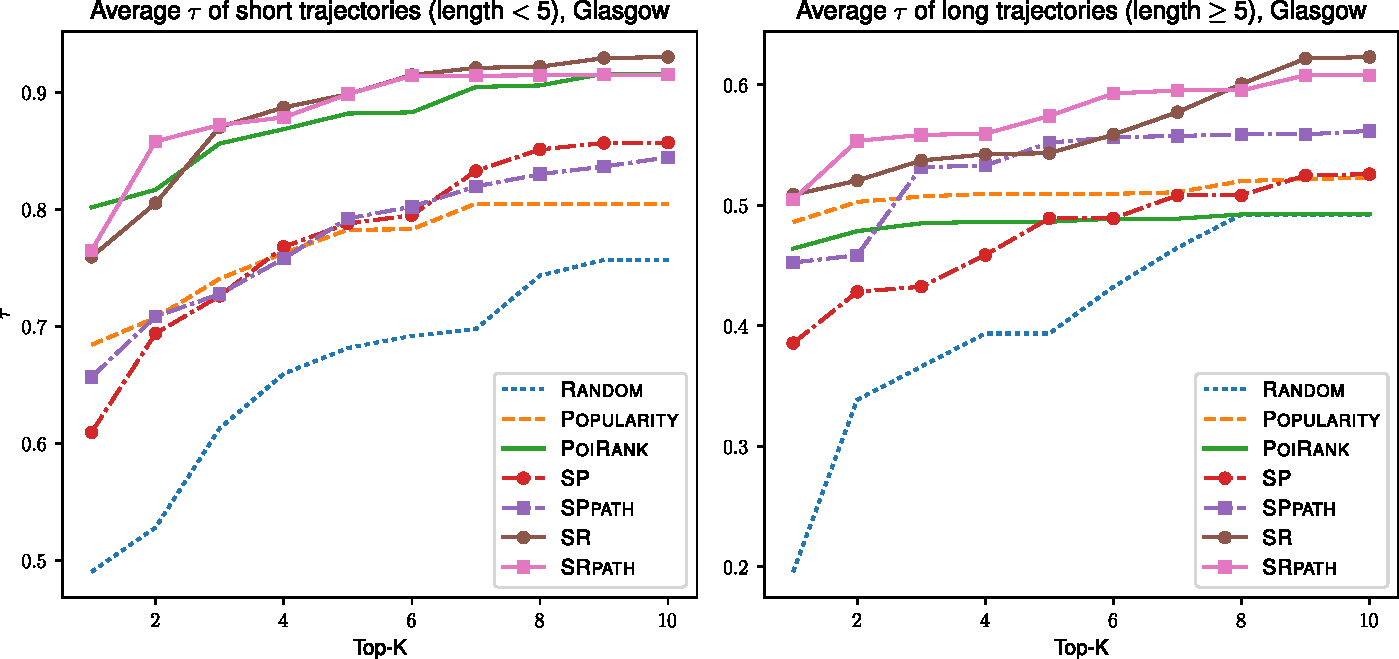
\includegraphics[width=0.65\linewidth]{tau_topk.pdf}
		%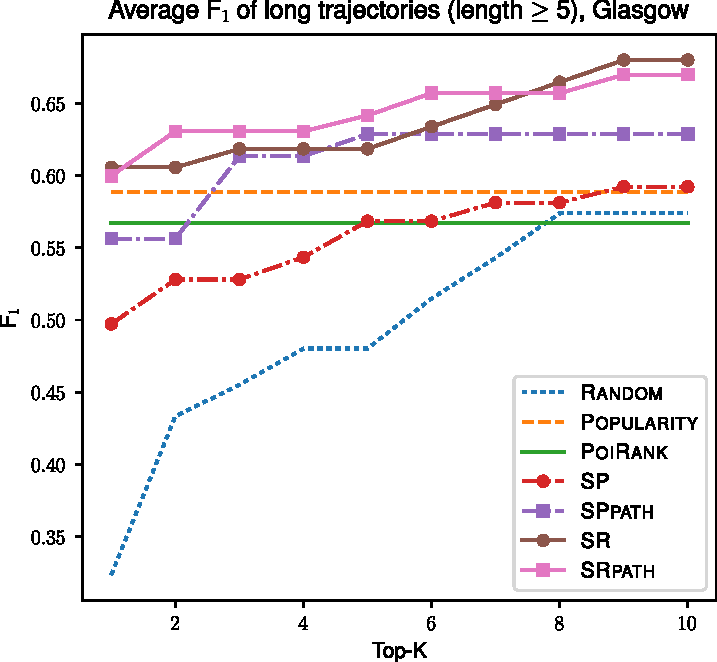
\includegraphics[width=0.33\linewidth]{f1_glasgow_gte5}
		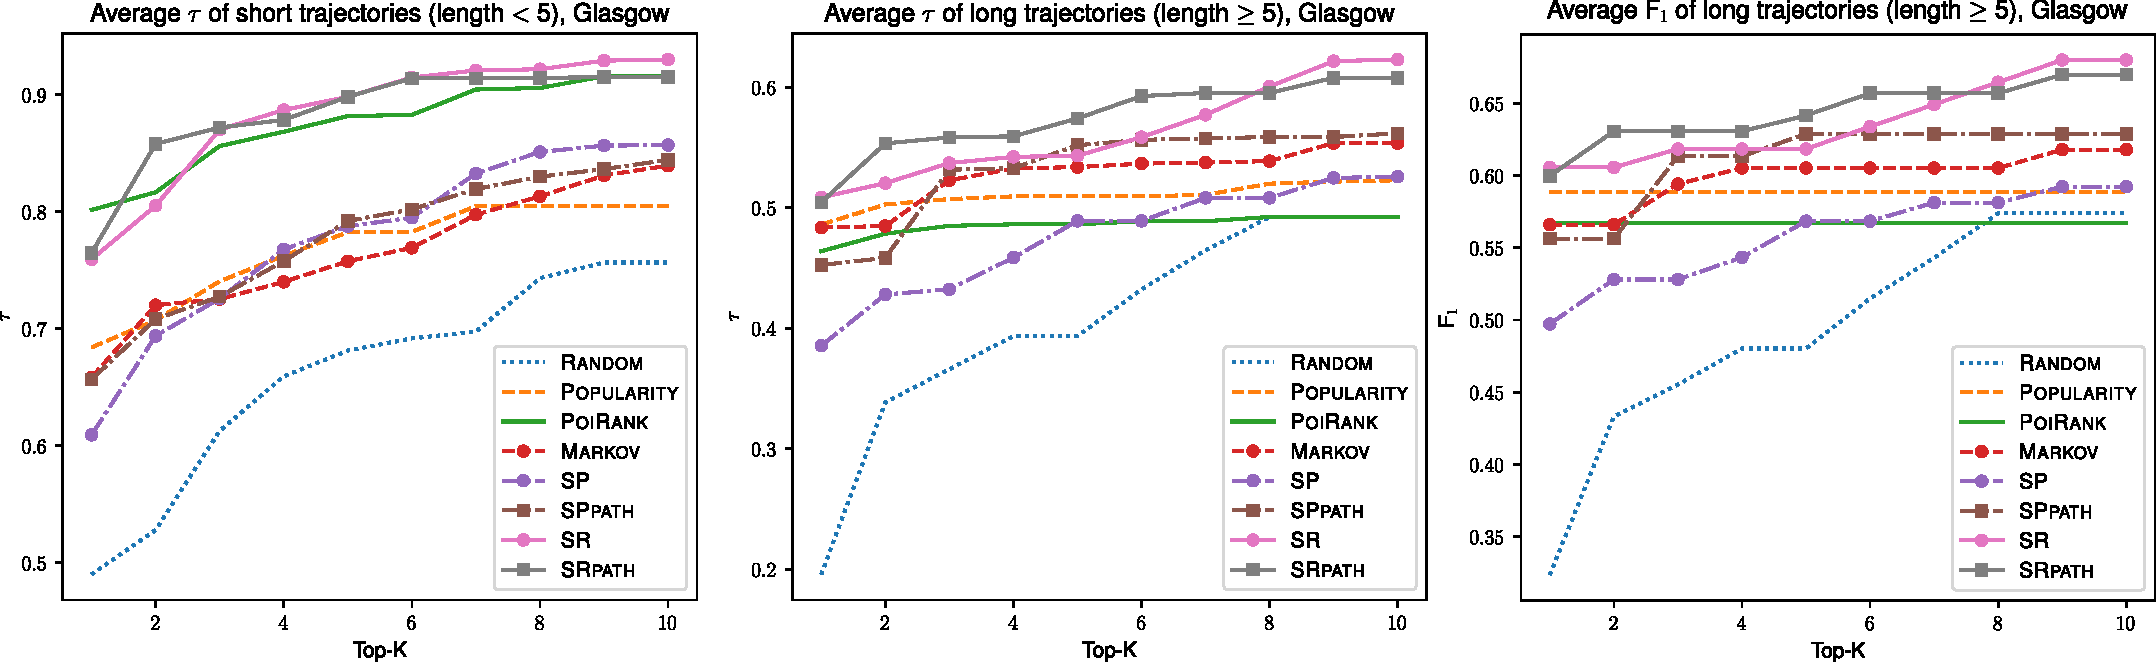
\includegraphics[height=0.33\linewidth]{performance_comp.pdf}
		}
	    \captionof{figure}{Average Kendall’s $\tau$ over $k=1\!:\!10$, for short (left) and long (middle) trajectories. (right) F$_1$ score on points for long trajectories.
			Sequence recommendation methods perform best for all values of $k$.
			For longer trajectories, the predictions of \textsc{Popularity} and \textsc{POIRank} are permutations of the same set of POIs (that do not fully overlap with the ground truth).}
	    \label{fig:topk}
	    %\captionmoveup\eqmoveup
\end{figure*}

% experimental results
%The performance of %three baselines and four variants based on structured prediction on two datasets
%all methods are shown in Table~\ref{tab:result}.


Table~\ref{tab:result} summarises the performance of all methods for top-10 recommendations.

\subsubsection{Is exploiting structure helpful?}
We can observe from the results that \textsc{POIRank}, \textsc{Markov} and \textsc{SP}
methods that convert the trajectory recommendation task
into data that is amenable to off the shelf methods (ranking, Markov chains and structured SVM respectively)
performs better than \textsc{Random} and \textsc{Popularity} baselines but are not the best performing methods.
Although \textsc{Markov} achieves the best performance on the smallest \texttt{Osaka} dataset,
the best results on larger datasets (\ie \texttt{Glasgow} and \texttt{Toronto}) are obtained using our proposed methods
%\textsc{SPpath}, 
\textsc{SR} and \textsc{SRpath}.


%\subsubsection{The performance in top-$k$ recommendation}
We also compare the performance for all values of top-$k$ with $k=1,\ldots,10$, and
Figure~\ref{fig:topk} shows a selection of the curves for \textsc{Glasgow}. We observe that
our proposed methods are consistently the best for all values of $k$.
See the supplement for results across all datasets on all metric variants.


%\subsubsection{Is eliminating multiple ground truths necessary?}
%\subsubsection{How important is it to account for multiple ground truths?}
\subsubsection{Is it important to account for multiple ground truths?}
%In particular,
%%\textbf{Exploiting the sequence structure helps}. The proposed structured recommendation variants of our achieve better performance than existing baselines.
%%Thus, the basis of our approach -- reducing sequence recommendation to a structured prediction problem -- is sensible, and has empirical benefit.
%Accounting for multiple ground truths helps --
We observe that \textsc{SR} always performs better than \textsc{SP},
and similarly for the {\sc path} variants of both methods.
This indicates that our first extension -- explicitly modelling multiple ground truths
 -- is important to achieve good performance.
%(We note that even without this correction, our structured methods outperform baselines.)
%LX - not sure we can claim this at all??
%\textbf{Eliminating loops during training helps}.
%{\sc SRpath} improves performance further of the {\sc SR} method,
%as indicated by the F$_1$ score on pairs.
%This indicates that our second extension -- explicitly performing sub-tour elimination in training -- is important to further improve performance.
%Interestingly,
%this advantage does \emph{not} take effect if the multiple ground truths are not modelled explicitly,
%with the performance of the {\sc SP} method largely unaffected.

%\subsubsection{When sequence recommendation perform best?}
We can also see that the advantages of {\sc SR} %, {\sc SPpath}, 
and {\sc SRpath} are salient for longer trajectories, where pairwise and sequential information play a larger role.

%\textbf{An illustrative example}.
%\rev{Figure~\ref{fig:example} illustrates with an example differences among the algorithms.} The query requires the trajectory to start from the point \rev{in the middle of the map} and be of length 3.
%\textsc{PoiRank} regards points at the lower right and upper left be of the highest rank, but did not consider their compatibility (\ie pairwise features). {\sc SP} and {\sc SR} hits one edge (green edge) out of the two ground truths, while {\sc SRpath} hits both edges for two valid trajectories by exploiting all factors.\TODO{dawei to make sure this example is sane, agrees w. eval protocol, and well-explained.}


%LX - reflections and confessions
Overall, sequence recommendation methods have shown superior performance in location sequence recommendation tasks on a public benchmark. Most notably, taking into account multiple ground truths in structured prediction and modeling path constraints are important; and the effects are more pronounced in longer trajectories.


%Finally, we note that the unary terms in the sequence scoring function \eqref{eq:jointfeature} can be replaced with {\em personalised} terms to each user, such as from a recommender system~\cite{Koren:2009,bpr09}. 
%We also note that the sequence recommendation problem suits well within the recurrent neural networks (RNNs) based techniques, 
%although these techniques generally require much more training data than available in our problem and 
%it is also not clear how to recommend a sequence as a whole instead of recommending the next best location as proposed in recent RNNs based work~\cite{aaai16}.
%We leave this and personalising sequence recommendation as future work.


%these results indicate that our structured prediction approach to the problem has
%benefits over non-structured approaches,
%and that our extensions to the vanilla structured approach are important to further improve performance.

\begin{figure}[htbp]
    \centering
    \begin{subfigure}[t]{.47\linewidth} % sub-figure environment width
        \centering
        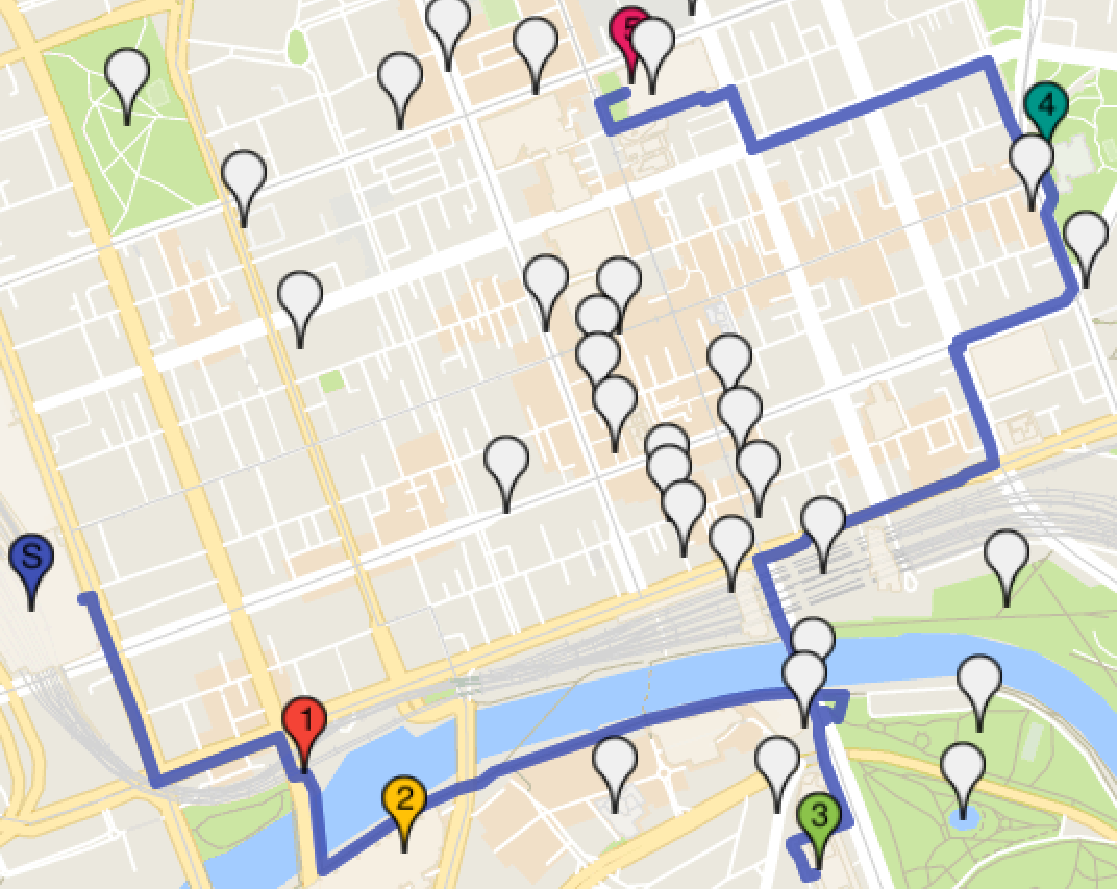
\includegraphics[width=\linewidth]{example_route.pdf}
        %\caption{}
        %\label{fig:route}
    \end{subfigure}
    \quad
    \begin{subfigure}[t]{.47\linewidth} 
        \centering
        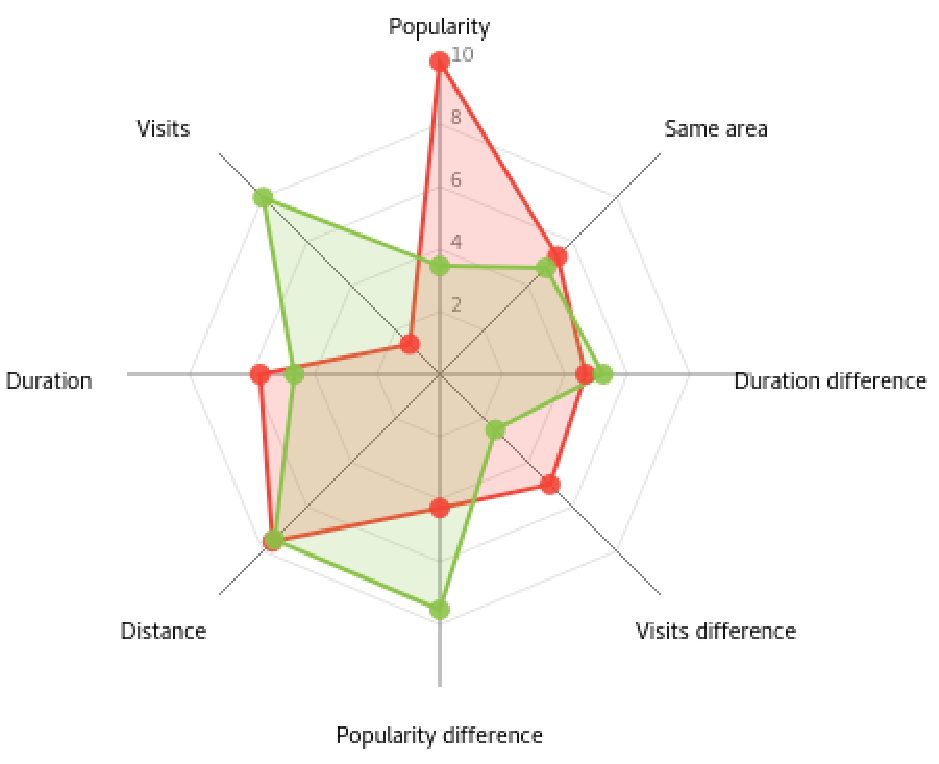
\includegraphics[width=\linewidth]{example_feature.pdf}
        %\caption{}
        %\label{fig:feature_comp}
    \end{subfigure}
    \caption{Example of a recommended trajectory (left); Radar charts that compare scores of two POIs decomposed according to features (right), see text for details.}
    \label{fig:example}
\end{figure}

\subsubsection{Example}
\label{sec:example}

Figure~\ref{fig:example} shows a recommended trajectory by the SR model, 
the trajectory includes 6 POIs and is visualised on a map (left);
the scores of two POIs are decomposed according to POI features (right),
in particular, the red radar chart shows the decomposition of the first POI (red marker on map) in the trajectory,
and the green chart shows the decomposition of the third POI (green marker on map).
We found that popularity and distance related features are the main contributors to the first POI,
and the third POI is largely supported by visits and distance related features.
%the left sub-figure visualises the trajectory on a map, 
%and the right sub-figure shows how different POI features contribute to the scores of two POIs using a radar chart.
%Figure~\ref{fig:example_sbar} uses a stacked bar plot to visualises the score decomposition of both POIs and transitions according to POI and pairwise features respectively.


%\begin{minipage}{0.5\linewidth}

%\begin{figure}[!h]
%    \centering
%    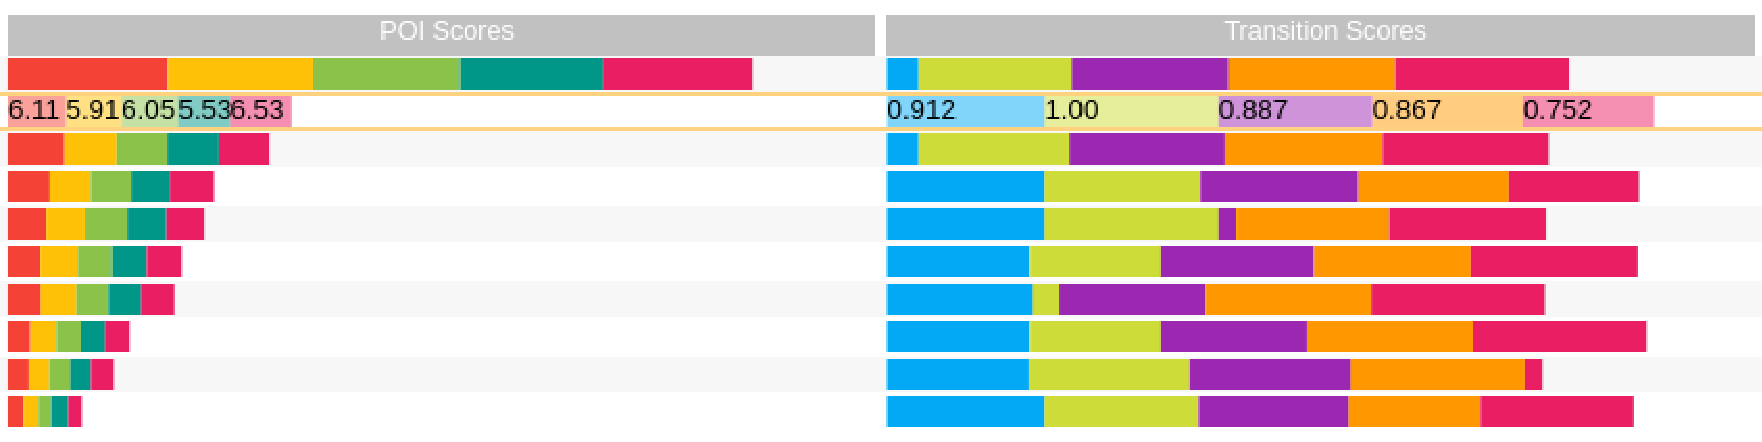
\includegraphics[width=\linewidth]{example_sbar.pdf}
%    \caption{A stacked bar plot compares scores of POI/transition decomposed according to features.}
%    \label{fig:example_sbar}
%\end{figure}

%\begin{figure*}[t]
%	\centering
%	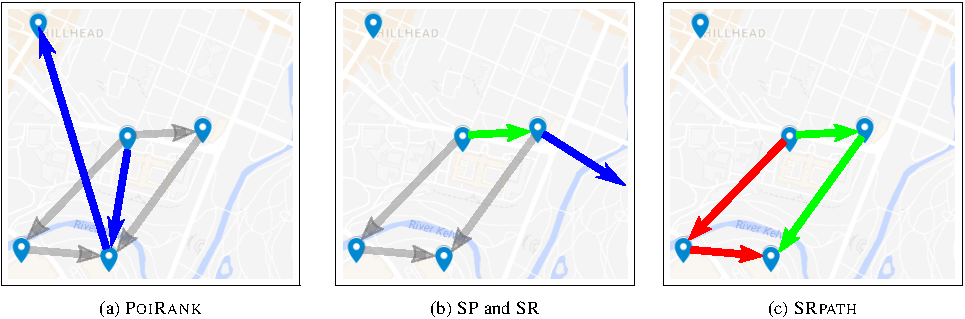
\includegraphics[scale=0.5]{example.pdf}
%	\caption{Example of structured recommender versus baseline on a query with two ground truths \rev{in Glasgow}. %as shown in Figure (c).
%             (a) \textsc{PoiRank} cannot make a recommendation related to any of the ground truths;
%             (b) \textsc{SP} and \textsc{SR} recommend a better trajectory than \textsc{PoiRank}, but not fully consistent with the ground truths;
%             (c) \textsc{SRpath} hits both ground truths at rank 3 (green edges) and 5 (red edges) respectively.}
%	\label{fig:example}\captionmoveup
%\end{figure*}
